\newpage
\hypertarget{m2ttex}{}
\subsection{Polishing the TGG Transformation}
\texHeader

\begin{itemize}

\item[$\blacktriangleright$] Open \texttt{NodeToDictionaryRule}, and add the following constraint to \texttt{dictionaryNode} as shown in
Fig.~\ref{eclipse:NodeToDictionaryRuleUpdated}.

\vspace{0.5cm}

\begin{figure}[htp]
\begin{center}
  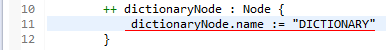
\includegraphics[width=0.7\textwidth]{eclipse_NodeToDictionaryUpdate}
  \caption[labelInTOC]{Updating \texttt{NodeToDictionaryRule}}
  \label{eclipse:NodeToDictionaryRuleUpdated}
\end{center}
\end{figure}


\item[$\blacktriangleright$] Similarly, open \texttt{ForAllEntryRule} and edit \texttt{entryNode} (Fig.~\ref{eclipse:ForAllEntryRuleUpdated}).\footnote{Please
note that the MOSL parser requires all attribute constraints to be declared before link variables.}

\vspace{0.5cm}

\begin{figure}[htp]
\begin{center}
  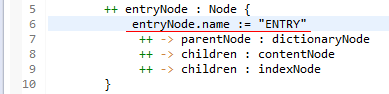
\includegraphics[width=0.7\textwidth]{eclipse_ForAllEntryRuleUpdated}
  \caption[labelInTOC]{Updating \texttt{ForAllEntryRule}}
  \label{eclipse:ForAllEntryRuleUpdated}
\end{center}
\end{figure} 

\item[$\blacktriangleright$] Now let's introduce our custom constraint to handle each \texttt{entryNode.index}
value. Update the \texttt{constraints} scope in \texttt{ForAllEntryRule} as shown in Fig.~\ref{eclipse:newEntryConstraint}.\footnote{ To review the purpose of
constraints and discuss the significance of each of the attribute options, refer to Part IV, Section 4.7.}

\vspace{0.5cm}

\begin{figure}[htbp]
\begin{center}
  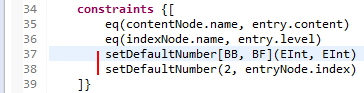
\includegraphics[width=0.7\textwidth]{eclipse_SetDefaultNumberConstraint}
  \caption{A final constraint for each \texttt{entry}}
  \label{eclipse:newEntryConstraint}
\end{center}
\end{figure}

\item[$\blacktriangleright$] That's everything! Save and build your updated \texttt{DictionaryCodeAdapter}, but don't run the TGG yet -- we haven't provided any
implementation for \texttt{setDefaultNumber}.

\end{itemize}
